\documentclass{standalone}
\usepackage{tikz,graphicx}
\usetikzlibrary{shapes,arrows,calc,positioning,backgrounds,plotmarks,plothandlers,fit}


\begin{document}

%\begin{tikzpicture}
%  \node[draw,rectangle] (A1) {$a_{1}$};
%  \node[draw,rectangle, below of=A1] (A2) {$a_{2}$};
%  \node[below of=A2] (ellipses) {$\vdots$};
%  \node[draw,rectangle, below of=ellipses] (An) {$a_{n}$};
%
%  \node[draw,rectangle, right= of A1] (GA1) {$GA$};
%  \node[draw,rectangle, right= of A2] (GA2) {$GA$};
%  \node[below of=GA2] (ellipses2) {$\vdots$};
%  \node[draw,rectangle, right= of An] (GAn) {$GA$};
%
%  \coordinate[right of = GA1] (rGA1);
%  \coordinate[right of = GA2] (rGA2);
%  \coordinate[right of = GAn] (rGAn);
%
%  \node[draw, rectangle, right= of rGA2] (result) {routes};
%
%  \node[above = of GA1] (lthreads) {Threads};
%  \node[above = of A1] (lagents) {Agents, $\mathcal{V}$};
%
%
%  \draw[->] (A1) -> (GA1);
%  \draw[->] (A2) -> (GA2);
%  \draw[->] (An) -> (GAn);
%
%  \draw[->] (GA1) -> (result);
%  \draw[->] (GA2) -> (result);
%  \draw[->] (GAn) -> (result);
%
%
%  \draw[thick,<->] (rGAn) -> node[left] {\tiny Shared Array} (rGA1);
%
%
%  \node[draw=red, fit=(GA1) (GAn) (rGAn)]  {};
%  \node[draw=blue, fit=(A1) (An)]  {};
%
%
%\end{tikzpicture}

%\begin{tikzpicture}[level/.style={sibling distance = 200cm/#1,
%  level distance = 18cm}]
%  \node [] {\includegraphics[]{images/bezint-1.png}}
%  child{
%    node [] {\includegraphics[]{images/bezint-2:1.png}}
%    child{
%      node [] {\includegraphics[]{images/bezint-3:1, 3.png}}
%      child{
%        node [] {\includegraphics[]{images/bezint-4:1, 3, 1.png}}
%        child{
%          node [] {\includegraphics[]{images/bezint-5:1, 3, 1, 3.png}}
%        }
%        child{
%          node [] {\includegraphics[]{images/bezint-5:1, 3, 1, 4.png}}
%          child{
%            node [] {\includegraphics[]{images/bezint-6:1, 3, 1, 4, 1.png}}
%          }
%          child{
%            node [] {\includegraphics[]{images/bezint-6:1, 3, 1, 4, 2.png}}
%            child{
%              node [] {\includegraphics[]{images/bezint-7:1, 3, 1, 4, 2, 3.png}}
%            }
%            child{
%              node [] {\includegraphics[]{images/bezint-7:1, 3, 1, 4, 2, 4.png}}
%              child{
%                node [] {\includegraphics[]{images/bezint-8:1, 3, 1, 4, 2, 4, 1.png}}
%              }
%              child{
%                node [] {\includegraphics[]{images/bezint-8:1, 3, 1, 4, 2, 4, 2.png}}
%              }
%            }
%          }
%        }
%      }
%      child{
%        node [] {\includegraphics[]{images/bezint-4:1, 3, 2.png}}
%        child{
%          node [] {\includegraphics[]{images/bezint-5:1, 3, 2, 3.png}}
%          child{
%            node [] {\includegraphics[]{images/bezint-6:1, 3, 2, 3, 3.png}}
%          }
%          child{
%            node [] {\includegraphics[]{images/bezint-6:1, 3, 2, 3, 4.png}}
%            child{
%              node [] {\includegraphics[]{images/bezint-7:1, 3, 2, 3, 4, 1.png}}
%            }
%            child{
%              node [] {\includegraphics[]{images/bezint-7:1, 3, 2, 3, 4, 2.png}}
%              child{
%                node [] {\includegraphics[]{images/bezint-8:1, 3, 2, 3, 4, 2, 3.png}}
%              }
%              child{
%                node [] {\includegraphics[]{images/bezint-8:1, 3, 2, 3, 4, 2, 4.png}}
%              }
%            }
%          }
%        }
%        child{
%          node [] {\includegraphics[]{images/bezint-5:1, 3, 2, 4.png}}
%          child{
%            node [] {\includegraphics[]{images/bezint-6:1, 3, 2, 4, 1.png}}
%          }
%          child{
%            node [] {\includegraphics[]{images/bezint-6:1, 3, 2, 4, 2.png}}
%            child{
%              node [] {\includegraphics[]{images/bezint-7:1, 3, 2, 4, 2, 3.png}}
%            }
%            child{
%              node [] {\includegraphics[]{images/bezint-7:1, 3, 2, 4, 2, 4.png}}
%            }
%          }
%        }
%      }
%    }
%    child{
%      node [] {\includegraphics[]{images/bezint-3:1, 4.png}}
%      child{
%        node [] {\includegraphics[]{images/bezint-4:1, 4, 1.png}}
%      }
%      child{
%        node [] {\includegraphics[]{images/bezint-4:1, 4, 2.png}}
%        child{
%          node [] {\includegraphics[]{images/bezint-5:1, 4, 2, 3.png}}
%        }
%        child{
%          node [] {\includegraphics[]{images/bezint-5:1, 4, 2, 4.png}}
%          child{
%            node [] {\includegraphics[]{images/bezint-6:1, 4, 2, 4, 1.png}}
%          }
%          child{
%            node [] {\includegraphics[]{images/bezint-6:1, 4, 2, 4, 2.png}}
%          }
%        }
%      }
%    }
%}
%  child{
%    node [] {\includegraphics[]{images/bezint-2:2.png}}
%    child{
%      node [] {\includegraphics[]{images/bezint-3:2, 3.png}}
%      child{
%        node [] {\includegraphics[]{images/bezint-4:2, 3, 3.png}}
%      }
%      child{
%        node [] {\includegraphics[]{images/bezint-4:2, 3, 4.png}}
%      }
%    }
%    child{
%      node [] {\includegraphics[]{images/bezint-3:2, 4.png}}
%      child{
%        node [] {\includegraphics[]{images/bezint-4:2, 4, 3.png}}
%        child{
%          node [] {\includegraphics[]{images/bezint-5:2, 4, 3, 1.png}}
%        }
%        child{
%          node [] {\includegraphics[]{images/bezint-5:2, 4, 3, 2.png}}
%          child{
%            node [] {\includegraphics[]{images/bezint-6:2, 4, 3, 2, 3.png}}
%          }
%          child{
%            node [] {\includegraphics[]{images/bezint-6:2, 4, 3, 2, 4.png}}
%          }
%        }
%      }
%      child{
%        node [] {\includegraphics[]{images/bezint-4:2, 4, 4.png}}
%      }
%    }
%  }
%  ;
%
%%  \node [below left = of p2-1] (p3-13) {\includegraphics[]{images/bezint-3:1, 3.png}};
%%  \node [below right = of p2-1] (p3-14) {\includegraphics[]{images/bezint-3:1, 4.png}};
%%
%%  \node [below left = of p2-2] (p3-23) {\includegraphics[]{images/bezint-3:2, 3.png}};
%%  \node [below right = of p2-2] (p3-24) {\includegraphics[]{images/bezint-3:2, 4.png}};
%
%
%\end{tikzpicture}

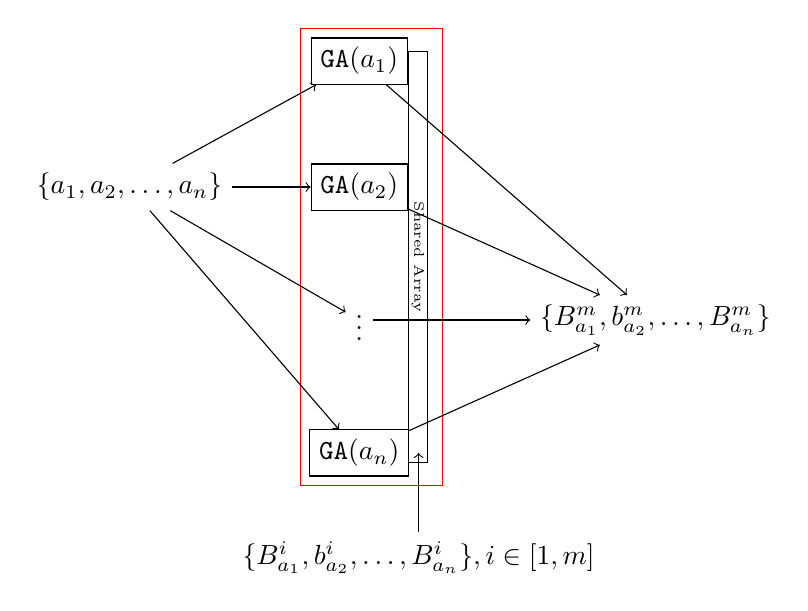
\begin{tikzpicture}
  \node[] (V) {$\{ a_{1}, a_{2}, \ldots, a_{n} \} $};

  \node[draw, rectangle, above right= of V] (ga1) {$\texttt{GA}(a_{1})$};
  \node[draw, rectangle, below = of ga1] (ga2) {$\texttt{GA}(a_{2})$};
  \node[below = of ga2] (gael) {$\vdots$};
  \node[draw, rectangle, below = of gael] (gan) {$\texttt{GA}(a_{n})$};

  \coordinate[right = 0.12of ga1.east] (rGA1);
  \coordinate[right = 0.2cm of rGA1] (rrGA1);
  \coordinate[right = 0.12cm of gan.east] (rGAn);

  \node[below = 1cm of rGAn] (sa) {$\{ B_{a_{1}}^{i}, b_{a_{2}}^{i}, \ldots, B_{a_{n}}^{i} \}, i \in [1,m] $};
  \node[right = 2cm of gael] (res) {$\{ B_{a_{1}}^{m}, b_{a_{2}}^{m}, \ldots, B_{a_{n}}^{m} \}$};

  \node[draw=black, fit=(rGA1) (rGAn), label={[rotate=-90]center:\tiny Shared Array}]  {};
  \node[draw=red, fit=(ga1) (gan) (rrGA1)]  {};

  \draw[->] (V) -> (ga1);
  \draw[->] (V) -> (ga2);
  \draw[->] (V) -> (gael);
  \draw[->] (V) -> (gan);

  \draw[->] (sa) -> (rGAn);

  \draw[->] (ga1) -> (res);
  \draw[->] (ga2) -> (res);
  \draw[->] (gael) -> (res);
  \draw[->] (gan) -> (res);
\end{tikzpicture}

\end{document}

%%% Local Variables:
%%% mode: latex
%%% TeX-master: t
%%% End:
